\section{Narrative Play}

Once you’ve made your engagement roll, prepared your gear and supplies, set your goal and your stakes, you’re officially on a mission. A mission could last one session or several sessions. You might abandon your original goal in favor of a new one, or encounter a twist in the story that throws your mission into disarray. Playing a mission out is mostly a matter of the GM - there’s no strong guidelines here as to how to structure it! However, here’s some tools, advice, and aid for running a mission.

                                     \textbf{Narrative play vs. mech combat} 

The following section deals with \textbf{narrative play,} typically when you’re using your pilot skills. This is the bit of the mission outside of mech combat, which is a lot more structured. Generally in narrative play each roll accomplishes much more, scenes can cover large stretches of time, and the outcome of individual rolls is more important.

\textbf{Mech combat} is turn based, tactical combat. Cutting to mech combat is as simple as declaring it’s started, drawing a map out, and picking who goes first. When you want each roll to accomplish more and want to play out turn based, tactical combat, you can swap to mech combat.

These are two different modes of play and the rules work slightly differently for each, especially combat. If you’re in narrative play and get into combat, you do combat with skill checks, and don’t make attack rolls. NPCs don’t get their own turns (nobody gets a ‘turn’ in narrative play), but their actions are narrated by the outcome of player rolls. If you’re doing mech combat, you use turn based, tactical play, make attack rolls and track hit points, and NPCs will take their own turns.

The rules for mech combat (and the difference from narrative play) are found right after the mech section.

\subsection{Making Skill Checks}

Skill checks are \textbf{only required when there is a tense narrative situation or when the check would move the story forward.} You don’t need to make a skill check to open a door, to cook a meal, or to talk to a superior, unless that situation is tense or would add to the story. You should generally always succeed on mundane tasks, especially if they relate to your background. A barroom brawl, a tense escape, decoding an encrypted message, hacking a computer, talking down a pirate, picking someone’s pocket, distracting a guard, hunting alien wildlife, or flattering the planetary governor are all situations that have some degree of tension and consequence, and might require a skill check.

Skill checks can cover as much or as little as the narrative requires. For example, you could have one skill check cover an entire day’s worth of infiltration into a covert facility if you so desire. Or, you could instead cover the moment to moment action - sneaking into vents, hacking doors, disabling guards, etc.

When making a skill check:\\
-    First name your goal.\\ 
-    The target number is always 10, and the check is a simple 1d20 roll. You then add any accuracy or difficulty from your skills, and then any accuracy or difficulty the GM imposes to get the total accuracy or difficulty on the roll.\\ 
-    You should only roll once to accomplish your goal (the GM can’t require extra rolls of you), though the GM could tweak the difficulty if you’re asking something very hard or complicated, or declare that given your goal or circumstances the roll would be impossible.\\ 
-    On a 9 or below, you don’t accomplish your goal. On a 10-19, you accomplish your goal. On a 20+, you excel on your goal.\\ 
-    On a 19 or lower, the GM can choose to add complications. 

Complications or consequences from failing or succeeding pilot skill checks\textbf{always follow the fiction and stakes established.} 


A failure doesn’t necessarily mean outright failure, but that you don’t directly accomplish your goal. Additionally, if you fail a check, you cannot attempt the same activity again until you change the narrative circumstances or approach (it’s a new day, you try something different). For example, you try to climb back up that cliff bare-handed, but fail. You could only make another skill check to climb the cliff again if you try it with a grappling hook, or get some other help.

                                                \textbf{Complications} 

On any result less than a 20+, the GM can throw additional complications or costs into the mix, \textbf{as established.} The GM doesn’t have to throw a complication in every time, and can just let the action play out - however rolling less than 20+ gives them the ability to do so. 

Complications are typically chosen from the categories of \textbf{Harm, Time, Resources, Collateral, Position, Effect.} This can n\textbf{ever nullify your success} if you roll a 10+ or cause you to not accomplish your goal, but can add additional nuance to the outcome of your skill check.


It’s important to note that the GM can only inflict complications if it makes sense to do so - in other words it must be \textbf{established} clearly before the roll. If you’re trying to take someone out with a sniper rifle at 500 meters and they have no way to see you or shoot back, you probably can’t take harm as a complication. If you’re trying to knock out a soldier from hiding that soldier probably doesn’t have a good way to fight back right away, even if you miss. If that soldier is alerted and looking for you, however, she might get a shot off.

-    \textbf{Harm} is damage, injury, or bodily harm, \textbf{as established.} If someone is pointing a gun at you, you attempt to take control of that gun and you fail, you will probably take harm.\\
-   \textbf{Time} means the activity takes more time than normal\\
-   \textbf{Resources} means something must be used up, lost, or temporarily expended. This could be something concrete like running out of ammunition, losing a map, or your gun jamming, or could be something like political influence.\\
-   \textbf{Collateral} means someone or something else takes harm or injury instead of you or your intended target, like an innocent bystander, the whole building, your organization or an ally\\
-   \textbf{Position} means you are put in a worse position through your actions, like right in the line of fire, clinging to the edge of a cliff, in the bad graces of the Baron, or under a spotlight\\
-   \textbf{Effect} means your action has less effect than you intend. If you were trying to take someone out cleanly, you make a lot more noise than you intended. If you try to fix a broken door, it will only open for a few people at a time. 

Narratively, complications are probably much worse if you fail (since you failed to accomplish your goal and got a complication). 

Example complications:\\
- \textbf{Harm:} A player rolls to knock someone out who just drew a knife on them by \textbf{applying fists to faces.} They don’t manage to knock their target out however, and they get a knife in the gut for 2 damage.\\
- \textbf{Time:} A player rolls to \textbf{charm} the baron into granting them an audience, succeeding. The baron lets them stew for a few hours, but gives them the audience.\\
- \textbf{Resources:} A player rolls to \textbf{patch} up an NPC’s wounds, and fails. The NPC not only bleeds out, but the player runs out of medical supplies trying to treat them.\\
- \textbf{Collateral:} A player rolls to \textbf{blow up} a door and fails. The whole building starts to collapse\\
- \textbf{Position:} A player rolls to \textbf{take out} an assassination target in a hidden base with a sniper rifle and succeeds. They kill their target, but they have to fire multiple times, exposing their position to the entire base.\\
- \textbf{Effect:} A player rolls to \textbf{wreck} a security system. It only shuts it down for 5 minutes, however, giving the players limited time to act.

                                                      \textbf{Excel} 

If you excel on a skill check (get a 20+), tell the GM how you surpass your initial goal. The GM can moderate this if it’s not within reason. In addition, the GM can’t throw complications at you - you did that well. 

Examples:\\
- \textbf{Bruja} excels when making a skill check to \textbf{hack} a door control. She suddenly finds herself with access to the whole network\\
- \textbf{Penny} excels when making a skill check to \textbf{threaten} a royal guard to stand down. The guard not only surrenders, but offers to help her get an audience with the king\\
- \textbf{Xi} excels when making a skill check to \textbf{get to the extraction point quickly.} He decides is able to find a shortcut to get the whole party there instead of just himself.\\
- \textbf{Raja} excels when making a skill check to \textbf{get a hold of} transport off world for his party. He decides that he manages to talk the shuttle pilot to walk off the job and hand the whole ship to his party

\subsubsection{Player Initiative and NPC Action}

Players \textbf{always have initiative} when making skill checks or taking action in narrative play. That’s a fancy way to say that the GM can never ask for a roll unless prompted by the players. Players must name their goal or aim of their action, then GMs can ask for a roll and set difficulty. When the roll is made, initiative turns back to the players (probably with a ‘what do you do?’ from the GM). What this does in practice is let players decide the course of action and make sure that each roll has clearly established stakes and parameters - it’ll help the game feel more fair and prevent unnecessary rolling. 

\textbf{If the players don’t take action,} stall, or pass off responsibility for action, then they are effectively\textbf{turning initiative over to the GM!} 

In addition, \textbf{NPCs} (non-player characters) don’t take actions or make rolls by themselves. Their actions are based on player rolls. For example, if a player lies to an NPC, the NPC doesn’t roll to see if the player is lying. If the player is successful, the NPC doesn’t see through their deception - if they fail, the NPC sees they are clearly lying. If the GM feels like the particular NPC is astute or insightful and can easily see through lies, they might add 1-2 difficulty to the roll.

There’s a little more on this in the GM section if you need examples. In practice you probably won’t even think about this that much.

\subsection{Skills in Detail}

Each skill has basic triggers that allow you to easily decide \textbf{which skill to use} and which bonuses from backgrounds or training \textbf{apply to a roll.} You don’t have to track or know all of them (just the ones which you have +accuracy or +difficulty in from backgrounds or training). If you’re stuck as to which skill you should be using, you can quickly refer to the triggers to get a good idea. 

Here’s a little more detail on each skill and when they might trigger. There’s intentionally a little overlap between some of the triggers, and each is designed to be somewhat flexible. \textbf{Remember, you don’t need to track all the skills, just the ones you are good or bad at!} 

\textbf{Applying fists to faces}\\ 
Punch someone in the face, or alternately fight in open, brutal unarmed combat, whether it’s a fist fight, martial arts duel, or a huge brawl. This is probably not the smoothest or cleanest fist fight and probably causes a lot of noise.

\textbf{Assault}\\
Take part in or direct an open or pitched battle, like a corridor gunfight, a huge shootout, fighting your way across a battlefield, or undertaking a boarding action. When you assault, you’re always assaulting something (a position, a rival pilot, an enemy force, a group of guards), and it’s always loud, open, direct action.

\textbf{Blow something up}\\
Use explosives (improvised or otherwise), weapons, or maybe just good old fashion brawn to totally wreck something or turn it into an enormous fireball (maybe a wall, sensor array, outpost, reactor core - the good stuff). Whenever you’re totally destroying an object, building, etc, you can use this. Probably not to be used against people unless they’re incidentally in the way.

\textbf{Threaten}\\
Use force or threats of force to get someone to do what you want them to do. Name what you want someone to do and what you’re going to do to them if they don’t listen to you. This could also be blackmail, leverage, or something similarly nasty. Threatening someone can be very high risk but very effective if successful. If you threaten someone unsuccessfully, your threats have no further effect on them unless you change something about the situation (like all other skill checks).

\textbf{Take control}\\
Use force, violence, presence of will, or direct action to take control of something. This is often something concrete, like an object someone is holding. You could take control of someone’s gun or a keycard they have on their person. You can additionally can take control of a situation to force those present to listen, calm down, stop moving, or stop what they’re doing, though you can’t necessarily force them to do anything further without threatening them. Taking control is never subtle and always direct and dangerous.

\textbf{Survive}\\
Persevere through harsh, hostile, or unforgiving environments, such as the vacuum of space, frozen tundra, a pirate enclave, a crime-ridden colony, untamed wilderness, or scorching desert. You most often use survive when you want to take a journey through wilderness environments, navigate, or avoid natural hazards such as carnivorous wildlife, rockfalls, thin ice, or lava fields. Alternately you could use it to avoid man-made hazards, such as navigating a city safely, or avoiding dangerous areas of a space station. You could also use it when testing personal endurance, such as shaking off poison or alcohol.

\textbf{Stay cool and collected}\\
Do something that requires concentration, speed, or intense precision under pressure, like picking a lock, finding the right frequency for your omnihook, carefully disarming an explosive, or unjamming a gun. If you’ve got to do something complicated in a high stress situation without messing up (and possibly not even breaking a sweat) this is the action to use. 

\textbf{Take someone out}\\
Kill or disable someone quickly, quietly, effectively or from a distance, probably before they even notice. This is probably a single person but could be two people relatively close together (any more is sort of stretching it). If you’re looking down a sniper scope at a target, preparing to nerve pinch a guard to knock them out instantly, quick-drawing during a gun duel, or dropping from a ceiling to slit a throat, this is the action to use.

\textbf{Flash}\\
Do something flashy, cool, or impressive with your weapon other than killing, like shoot a very small or rapidly moving target, shooting someone’s hat off or their weapon out of their hand, knocking someone out by throwing a gun at them, performing an acrobatic flourish with a sword, throwing a spear to pin a fleeing target to the ground, or something similar.

\textbf{Get somewhere quickly}\\
Get somewhere without complications and with speed, but not necessarily quietly. Climb, swim, or perform acrobatic maneuvers. Fall safely from a great height. Move gracefully in zero-g. Chase or flee from, outrun or out pace a target. Get somewhere faster than anyone else. You can also use this when you want to drive or pilot a vehicle.

\textbf{Act unseen or unheard}\\
Get somewhere or do something without being detected, but not necessarily with speed. Hide, sneak, or move quietly. Infiltrate a facility while avoiding security, patrols, or cameras. Perform a quick action or maneuver without being seen or heard, such as picking a pocket, unholstering your gun, or cheating at cards. Wear a disguise.

\textbf{Fix, hack, or wreck}\\
Repair a device or faulty system. Alternately, hack it wide open, or totally wreck, disable or sabotage it. You can use this for hacking or safeguarding electronic systems, such as electronic door locks, computer systems, omninet webs, or NHP coffins.

\textbf{Patch}\\
Apply your medical knowledge to administer medication, bandage, staunch bleeding, suture, cauterize, neutralize poison, or resuscitate. Alternately, you could use it to diagnose or study disease, pathogens, or illness.

\textbf{Invent or create}\\
You need tools and supplies to invent or create something successfully. Use this with many downtime actions to work on projects. You can also use it in the spur of the moment to invent new devices, tools, or approaches to something (improvised explosives, gear, disguises, or some similar).

\textbf{Read a situation}\\ 
Look for subtext, motive, or threat in a situation or person, often social situations. Use your intuition to learn someone’s motivation, who is really in charge, or who is about to do something rash or stupid. Get a gut feeling about a situation or person. Sense if someone is lying to you.

\textbf{Spot}\\
Spot hidden or difficult to make out details, objects, or people. Spot ambushes, hidden compartments, or disguised individuals. Spy on a target from a distance, or make out the details, shape, and number of objects, vehicles, mechs, or people clearly at a distance. Track people or vehicles.

\textbf{Investigate}\\
Research a subject, or look at something in great detail. If you can’t find information directly, you learn how you can get access to that information. Learn about a subject of historical relevance, or become well-read on a subject. Investigate a mystery or solve a puzzle. Locate a person or object through research or investigation.

\textbf{Charm}\\
To charm, you need a receptive audience, or some kind of promise of leverage (money, power, personal benefit, etc). You can use it when trying to smooth talk your way past guards, get someone on your side, sway a potential benefactor, talk someone down, perform diplomacy between two parties, or blatantly lie to someone. You can also use it when trying to impersonate someone. Charm won’t work on people that aren’t receptive (such as soldiers you are in a gunfight with) or that you don’t have leverage over (promises of safety, money, power, recompense, help, etc). These promises don’t necessarily have to be true but they have to have some weight with your target.

\textbf{Pull Rank}\\
Pull rank on a subordinate, getting information, resources, or aid from them, even unwillingly. You can use this on anyone your social status (noble, celebrity, etc) or military rank would have weight with. Failing this might be risky and could be seen as abusive. You typically can’t pull rank on hostile targets. You could also use this to pull rank and pretend you are a higher rank than you are, but it’s even riskier.

\textbf{Word on the streets}\\
Get gossip, news, or hearsay from the streets. What you get depends on what ‘streets’ you are getting word from (high society, low society, hearsay, military chatter, etc). This probably takes a lot less time than investigating something in detail, but the information might be more qualitative or colored by opinion (sometimes that might be useful). You can always learn where the information came from or who to go to next.

\textbf{Get a hold of something}\\
Acquire useful allies, assets, or connections through wealth or social influence. This could be permanent (buying it or receiving it) or temporary (renting or borrowing help or supplies, etc), and might be harder or easier depending on how much you want to use it. This can’t be used for something that’s normally gated by license level (like mech parts) but could be used for aid, supplies, information, food materials, soldiers, or anything else that has more narrative impact. Typically this is acquired by buying it from a market or requisitioning it from a parent organization.

\textbf{Lead or inspire}\\
Give an inspiring speech, or motivate a group of people into action. Administer or run an organization efficiently or effectively, such as a company, a ship’s crew, a group of colonists or a mining venture. Effectively command a platoon of soldiers in battle, or (perhaps) an entire army.

\subsubsection{Skill Challenges}

A skill challenge is a simple way to test an entire group for a particular activity. Everyone makes a
relevant check, and the success of the challenge depends on the overall result of the skill checks
from the entire group, not just one player. If more players succeed than fail, the challenge is a
success. If equally as many succeed as fail, the challenge has a 50\% chance of success (roll a
die or flip a coin), representing the razor’s edge of the situation. If more players fail than succeed,
the challenge is a failure.

Here’s some example challenges:\\
-    \textbf{Sneaking into a guarded facility:} All players roll a skill check (example skills that could trigger: \textbf{move unseen,} \textbf{spot} the cameras, \textbf{charm} the guards into thinking they are a superior). Success means they all get in unnoticed, failure means the guards are alerted.\\
-    \textbf{Gaining the favor of the Baron:} All players roll a skill check (example skills that could trigger: \textbf{charm,} but could also be to \textbf{threaten} the baron, or perhaps \textbf{read the situation}) Success means the players gain a private audience with the Baron, failure means the players’ meddling is noticed by rival nobility and they are thrown out.\\
-    \textbf{Traversing the Wastes:} All players roll a skill check (example skills that could trigger: \textbf{survive,} \textbf{spot} water, or \textbf{get} across the waste \textbf{quickly}). Success means they cross the wastes unharmed. Failure means they cross the wastes, but it is a harrowing journey and they arrive there with no repairs or supplies left and lacking food and water.

Challenges are good when you want to extend the narrative impact of rolls.

You can also have extended challenges that have \textbf{3 rounds} of rolling and calculate the outcome based on rounds ‘won’ by the players. For example, the players may have to gain the favor of the baron, then plant information in the baron’s castle, and sabotage the gate. They are only truly successful if the majority (2/3) of these tasks are accomplished.

\subsection{Combat in Narrative Play}

When running combat \textbf{narratively}, use the normal rules for skill checks. That means when the individual actions in combat doesn’t matter that much or you want a combat scene to play out more like a movie than a tactical game. If there’s not a mech involved (and you’re just playing on the pilot scale), it’s almost always preferable to use narrative combat.

You don’t need to track turns or make attack rolls, and you might only need to make a few rolls for the whole combat (one roll for each action or goal, as normal!). Turn-based combat in LANCER is usually reserved for mech combat.

You can also use a skill challenge to run narrative combat if you want it to be a bit more structured. 

Here’s a couple examples:\\
- \textbf{Bruja} and \textbf{Penny} are negotiating with the Black Star Bandits to try and get them to release a hostage. The negotiations go sour (Penny fails her skill check to \textbf{charm} the bandit captain), and the bandits draw on them. Bruja decides to \textbf{take out} the bandits quickly with her Sidekick. She rolls a skill check, getting a 15. She kills the bandits and the GM decides to add position as a complication, so the rest of the bandit camp is alerted and they will need to get out quickly.\\
- \textbf{Pan} is in a pitched battle, on foot. He sees a gun emplacement raining hell down upon his allies and decides to \textbf{take control} of it. He rolls and gets a 7, failing. The soldiers defending the emplacement turn the gun on him, preventing him from getting any closer. The GM adds \textbf{collateral} as a complication. Pan looks behind him and sees some members of his squad get gunned down in the ill-advised assault.\\
- \textbf{Raja} is commanding a platoon of troops to board an enemy ship and take control of the command center. He rolls to \textbf{lead} the charge, getting a \textbf{22}, (he excels). There’s no complications, and when his group successfully fights their way to the command center, they immediately surrender and hand control over.

\newpage
\begin{center}
  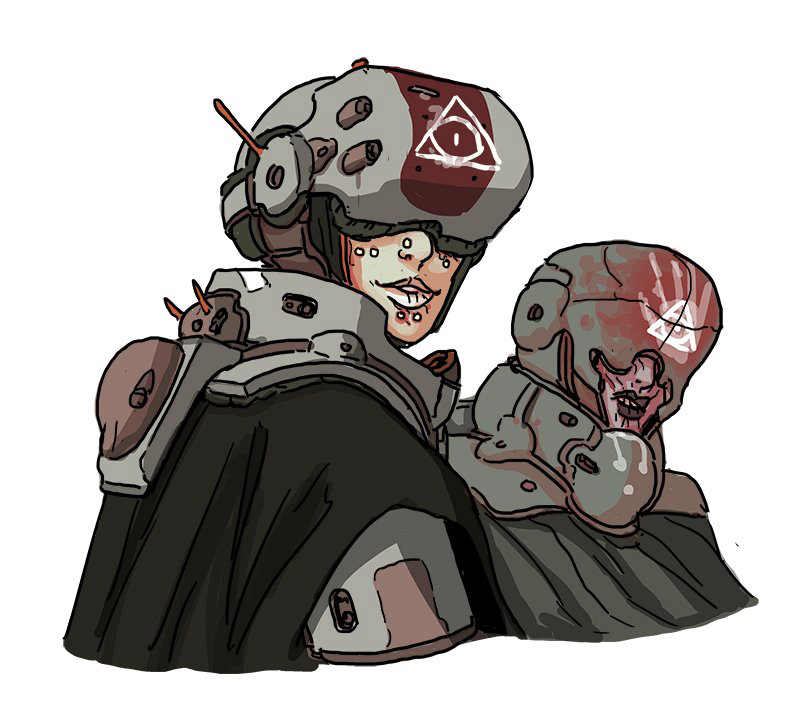
\includegraphics{Ungratefuls}
\end{center}
\subsubsection{Hit Points, Damage, and Injury}

Pilots normally only care about Hit points, also called HP (how much damage your pilot can take before they are out of the action!) during mech combat, but they might also take damage as a result of complications during skill checks.

At level 0, pilots have \textbf{6 Hit Points,} representing not only bodily health, but also the ability to duck, dodge, avoid damage, or just sheer luck. At higher levels, they add their \textbf{grit (1/2 level)} to calculate their base HP (leading to a total of 6 + grit). A pilot that takes damage \textbf{doesn’t necessarily take bodily harm,} but might be using up their stamina, luck, or ability to avoid that incom- ing damage.

If a consequence deals damage, it’s enough to hurt or kill. Taking things like minor grazes, bruises, etc doesn’t deal damage but could cause other complications.

Here’s what damage looks like for pilots in narrative play:\\
\textbf{Minor} damage is 1-2 damage. This could be something like getting shot at by small arms fire, stabbed, unarmed combat, hit by a flying rock, etc\\
\textbf{Major} damage is 3-4. This is getting shot at by assault or heavy weapons, a long fall, breathing in toxic gas, etc\\
\textbf{Lethal} damage is 6+. This is something like having a mech fall on you, getting hit by a mech scale weapon, having a grenade blow up right under you or something similar.

Pilots might have 1 or 2 armor. Subtract armor from all damage taken as a pilot, unless that damage has the armor piercing (ap) tag. Some weapons have the ap tag, but damage outside of that might also (falling a long distance, being immersed in lava, etc).

                                                \textbf{Down and out} 

If you’re reduced to 0 HP or lower as a pilot roll a 1d6. On a 6, you miraculously shrug off the hit (or its a close call), returning to 1 HP. If you roll a 1, your luck has run out, and you’re immediately dead. If you roll a 2-5, you are \textbf{down and out, at 0 HP.} You’re knocked out, pinned, bleeding out, or otherwise unable to act. Your evasion (how hard it is to hit you in mech combat) becomes 5 and if you take any more damage, you’ll die (if someone comes over and shoots you in the head, for example).

You can die instead of being down and out, if you choose so. Typically you’d just bleed out and wake up in prison, a field camp, a hospital, or buried under a pile of dead bodies somewhere.

\subsubsection{Rests and Full Repair}

If a character takes an hour and \textbf{rests} with no strenuous activity, they can regain 1/2 their HP, and recover from Down and Out, coming back to consciousness. When you take at least 10 hours to rest and \textbf{full repair}, you can recover all your hp. 

Rest and repair also help your mech (you can see more in the mech section on damage). 

If you’re \textbf{dead}, it might not be the end for you. See the rules on cloning in the Death section in mech combat.